\documentclass[a4paper,11pt]{article}

\usepackage[T1]{fontenc}
\usepackage[utf8]{inputenc}
\usepackage{graphicx}
\usepackage{xcolor}
\usepackage[italian]{babel}
\selectlanguage{italian}


%% Useful packages
\usepackage{amsmath}
\usepackage{graphicx}
\usepackage{graphics}
\usepackage[colorinlistoftodos]{todonotes}
\usepackage[colorlinks=true, allcolors=blue]{hyperref}
\usepackage{csquotes}
\usepackage{amsmath,amssymb,amsthm,textcomp}
\usepackage{enumerate}
\usepackage{multicol}
\usepackage{tikz}

%___________________Sets page size and margins___________________%
\usepackage{geometry}
\geometry{left=25mm, right=25mm, top=20mm, bottom=20mm}

\newcommand{\linia}{\rule{\linewidth}{0.5pt}}


%______________________Listing________________________%


\usepackage{listings}
\usepackage{color}

\definecolor{codegreen}{rgb}{0,0.6,0}
\definecolor{codegray}{rgb}{0.5,0.5,0.5}
\definecolor{codepurple}{rgb}{0.58,0,0.82}
\definecolor{backcolour}{rgb}{0.95,0.95,0.92}

\lstdefinestyle{mystyle}{
    language=Java,
    aboveskip=5mm,
    belowskip=5mm,
    columns=flexible,
    backgroundcolor=\color{backcolour},   
    commentstyle=\color{codegreen},
    keywordstyle=\color{magenta},
    numberstyle=\tiny\color{codegray},
    stringstyle=\color{codepurple},
    basicstyle=\ttfamily\footnotesize,
    breakatwhitespace=false,         
    breaklines=true,                 
    captionpos=t,                    
    keepspaces=true,                 
    numbers=left,                    
    numbersep=5pt,                  
    showspaces=false,                
    showstringspaces=false,
    showtabs=false,                  
    tabsize=2
}

\lstset{style=mystyle}



%______________________Listing________________________%
\usepackage{tcolorbox}
\tcbuselibrary{theorems}

\newtcbtheorem{mytheo}{Osservazione}%
{colback=green!5,colframe=green!35!black,fonttitle=\bfseries}{th}


%______________Team's comments______________%

\newcommand{\stefano}[1]{{\bf \color{red} Stefano: #1 }}
\newcommand{\andrea}[1]{{\bf \color{teal} Andrea: #1 }}
\newcommand{\davide}[1]{{\bf \color{chromeyellow} Davide: #1 }}

\usepackage[sorting=none, isbn=false, eprint=false]{biblatex}
\addbibresource{bibliography.bib}


\begin{document}

\begin{figure}
    \centering
    
\includegraphics[width=0.25\linewidth]{immagini/unito_logo.jpg}
\end{figure}

\begin{center}
    \vspace{5ex}
    {\huge \textbf{Esame di Java}}
    \vspace{1ex}
    \linia
    \vspace{3ex}
\end{center}

\begin{center}
 Davide Marietti, Università di Torino
\end{center}
\begin{center}
    Andrea Balbo Mossetti, Università di Torino
\end{center}

\vspace{5ex}

\begin{center}
    Master IT Full Stack Design and Development, a.a. 2022/2023

\end{center}

\newpage
	\tableofcontents
    \lstlistoflistings
	
\newpage


\section{Descrizione del lavoro}

Per la realizzazione della consegna siamo partiti dalla traccia fornita dalla Professoressa, con cui venivamo invitati ad implementare uno \textit{Shelter} per animali. Questo progetto riguarda il corso di Java base. Pertanto, ci siamo concentrati sullo sviluppo dei concetti base della programmazione ad oggetti vista a lezione, piuttosto che sull'implementazione di funzionalità complesse che utilizzino librerie esterne. Tutte le funzionalità implementate utilizzano esclusivamente oggetti della libreria Standard di Java \cite{java_lib}. Abbiamo cercato di includere nel codice i concetti fondamentali della programmazione ad oggetti in Java, il che ci ha permesso di ragionare sui concetti di \textbf{binding dinamico}, \textbf{classi astratte}, \textbf{sottoclassi}, \textbf{upcasting}, \textbf{sovratipo}, \textbf{array di oggetti}, \textbf{overloading} \textbf{ereditarietà}, \textbf{overwriting}, \textbf{information hiding}, \textbf{security leaking}~\cite{java}\cite{java_book}.


\section{Classi implementate}
Il codice seppur minimale, nasconde al suo interno spunti interessanti.


\subsection{Classe Animal}

Il primo passo \'e quindi consistito nell'allestimento di una classe {\tt Animale}, che astrae il concetto di animale. La classe è definita \textbf{astratta} per due principali motivi:
\begin{itemize}
    \item Non posso definire un oggetto con tipo esatto {\tt Animal}, quindi ciascun animale deve essere definito attraverso una delle sottoclassi \textbf{concrete} di {\tt Animal} \cite{java}.
    \item Avere una sovraclasse comune (e obbligata) per ciascuna specie di animale ci consente di usate l'\textbf{upcasting} per poter definire una array di oggetti di tipo {\tt Animal} che ci permette di astrarre il concetto di shelter \cite{java_book}.
    \item La definizione del metodo {\tt equals} ci ha permesso di discutere il concetto di {\em uguaglianza} tra oggetti.
\end{itemize}

\begin{lstlisting}[caption={Animal.java -- Allestimento della classe Animale}]
abstract class Animal {
 	private String name, breed;
   private int age, conditions; // condizioni di salute dell'animale adottato

	// costruttore
   public Animal(String breed, int age, int conditions) {
  this.breed = breed;
  this.age = age;
  this.conditions = conditions;
   }


// some methods here 
}

\end{lstlisting}

Abbiamo definito animali appartenenti a specie specifiche, sfruttando la possibilit\'a di estendere la suddetta classe. In questo modo, le specie di animali che stiamo andando ad implementare erediteranno gli attributi che abbiamo definito poco sopra e ne specificano di nuovi per aumentare il dettaglio di astrazione dell'animale.

Notare che per ciascun animale è indicato anche il suo stato di salute al momento dell'ingresso nello shelter. Lo scopo dello shelter è anche quello di curare gli animali, oltre che ospitarli. Alleghiamo codice esemplificativo:

\begin{lstlisting}[caption={Aniaml.java -- Estensione della classe {\tt Animal} per definire nuove specie.}]
class Dog extends Animal {

// Subclasses add more feature alla classe che specializzano
private String size;

public Dog(String breed, int age, String size, int conditions) {
  super(breed, age, conditions);
  this.size = size;
}

public Dog(String name, String breed, int age, String size, int conditions) {
  super(name, breed, age, conditions);
  this.size = size; // NB: this esplicito
}

// OVERWRTING del metodo toString()
public String toString() {
  String s = super.toString() + ", taglia: " + size + ", animale: cane"; // NB: this implicito

  return s;
}
}


class Cat extends Animal {
private boolean longFur;

public Cat(String breed, int age, boolean longFur, int conditions) {
  super(breed, age, conditions);
  this.longFur = longFur;
}

public Cat(String name, String breed, int age, boolean longFur, int conditions) {
  super(name, breed, age, conditions);
  this.longFur = longFur;
}

public String toString() {
  String s = super.toString() + ", pelo lungo: " + longFur + ", animale: gatto";;

  return s;
}
}

\end{lstlisting}

Notiamo alcuni aspetti interessanti:
\begin{itemize}
    \item Innanzitutto l'\textbf{overloading} del costruttore di ciascuna sottoclasse.
    \item L'\textbf{overwriting} del metodo {\tt toString()}, il quale appartiene alla superclasse {\tt Object}, e viene specializzato per ciascuna animale.
\end{itemize}

L'overloading del costruttore permette di inizializza gli animale già con un nome, oppure, se ``trovatelli'', di dargli un nome al momento del loro insediamento nello shelter.


\subsection{Classe AnimalShelter}

\begin{lstlisting}[caption={AnimalShelter.java}]
public class AnimalShelter {
   private int nAnimals = 0; // inizialmente lo shelter non contiene animali
   private Animal[] hostedAnimals;

   // Definisco lo shelter come un array di oggetti, quindi avente una capienza limitata a maxNumAnimals
   public AnimalShelter(int maxNumAnimals) {
      hostedAnimals = new Animal[maxNumAnimals];
   }

   // Converto l'astrazione dell'AnimalShelter in una stringa. Notare la chiamata al metodo toString della classe Animal.
   public String toString() {
      String s = "Numero di animali ospitati = " + nAnimals;

      int i = 0;
      while (i < nAnimals) {
         s = s + hostedAnimals[i].toString();
         ++i;
      }

      return s;
   }

   public int getNumAnimals() {
      return nAnimals;
   }

   public int findHostedAnimalIndex(String name) {
      int i = 0;
      while (i < nAnimals) {
         if (hostedAnimals[i].getName().equalsIgnoreCase(name)) return i;
         ++i;
      }

      return nAnimals;
   }

   public boolean checkIfPresent(String name) {
      return (findHostedAnimalIndex(name) < nAnimals);
   }

   public boolean checkIfFull() {
      return (nAnimals == hostedAnimals.length);
   }

   public boolean hostAnimal(Animal animal, String name) {

      if (checkIfFull()){
         return false; // Se lo shelter è pieno il motodo fallisce
      }

      animal.setName(name);
      hostedAnimals[nAnimals] = animal;
      ++nAnimals; // aggiorno il numero degli animali presenti

      return true;
   }

   public boolean animalAdopted(String name) {
      int i = findHostedAnimalIndex(name);
      if (i == nAnimals) {
         return false; // se l'animale non esiste il motodo fallisce
      }

      --nAnimals;
      hostedAnimals[i] = hostedAnimals[nAnimals];

      return true;
   }
}
\end{lstlisting}

L'astrazione dello shelter avviene tramite la definizione di un array di animali e dei relativi metodi {\tt hostAnimal(...)} e {\tt animalAdopted(...)}. Come accennato in precedenza, un array in Java deve contenere oggetti aventi lo stesso tipo apparente, per questo sfruttiamo il \textbf{binding dinamico} definendo ciascun animale con tipo apparente {\tt Animal} e con tipo esatto quello specifico della specie.
Notare:
\begin{itemize}
    \item come l'\textbf{information hiding} sia stato opportunamente implementato per non dare accesso diretto all'array di animali, ma consentendo di interagire con esso tramite gli opportuni metodi pubblici\cite{java},
    \item come il metodo {\tt toString()} venga anche qui ridefinito tramite overwriting \cite{java},
    \item come il concetto che lo shelter debba avere un numero di posti limitato venga preso in carico dalla variabile privata {\tt nAnimals}, che definisce la lunghezza dell'array di animali \cite{java_book}. Un array in Java ha infatti una lunghezza fissata al momento del suo ``instanziamento'' nella heap.
\end{itemize}


\subsection{Classe User}

La classe {\tt User} è molto semplice e permette di astrarre la figura dell'utente che interagisce con lo shelter nell'adottare e nel curare gli animali.

\begin{lstlisting}[caption={AnimalShelter.java}]
public class User {
   private String name;
   private String surname;
   private String email;
   private String cell;

   public User(String name, String surname, String email, String cell){
      this.name = name;
      this.surname = surname;
      this.email = email;
      this.cell = cell;
   }

   public boolean adoptAnimal(AnimalShelter shelter, String name){
      return shelter.animalAdopted(name);
   }

   public void cureAnimal(Animal animal){
      animal.setConditions(100);
   }
}
\end{lstlisting}

Notare come lo user non agisce direttamente sull'oggetto {\tt AnimalSherlter}, ma solo tramite i metodi pubblici di {\tt AnimalSherlter}, in questo modo si evitano possibili problemi di \textbf{security leaking}.

Un esempio di utilizzo delle classi sopracitate ci è fornito dal client {\tt DemoAnimalShelter.java} riportato in appendice \ref{appendice:A}. Sempre in appendice \ref{appendice:A}, in figura \ref{fig:output} si può osservare il semplice e chiaro output del client.

Una rappresentazione della connessione delle classi brevemente descritte qui sopra e presentata sotto forma di diagramma UML in figura \ref{fig:UML}.

\begin{figure}[!t]
    \makebox[\textwidth][c]{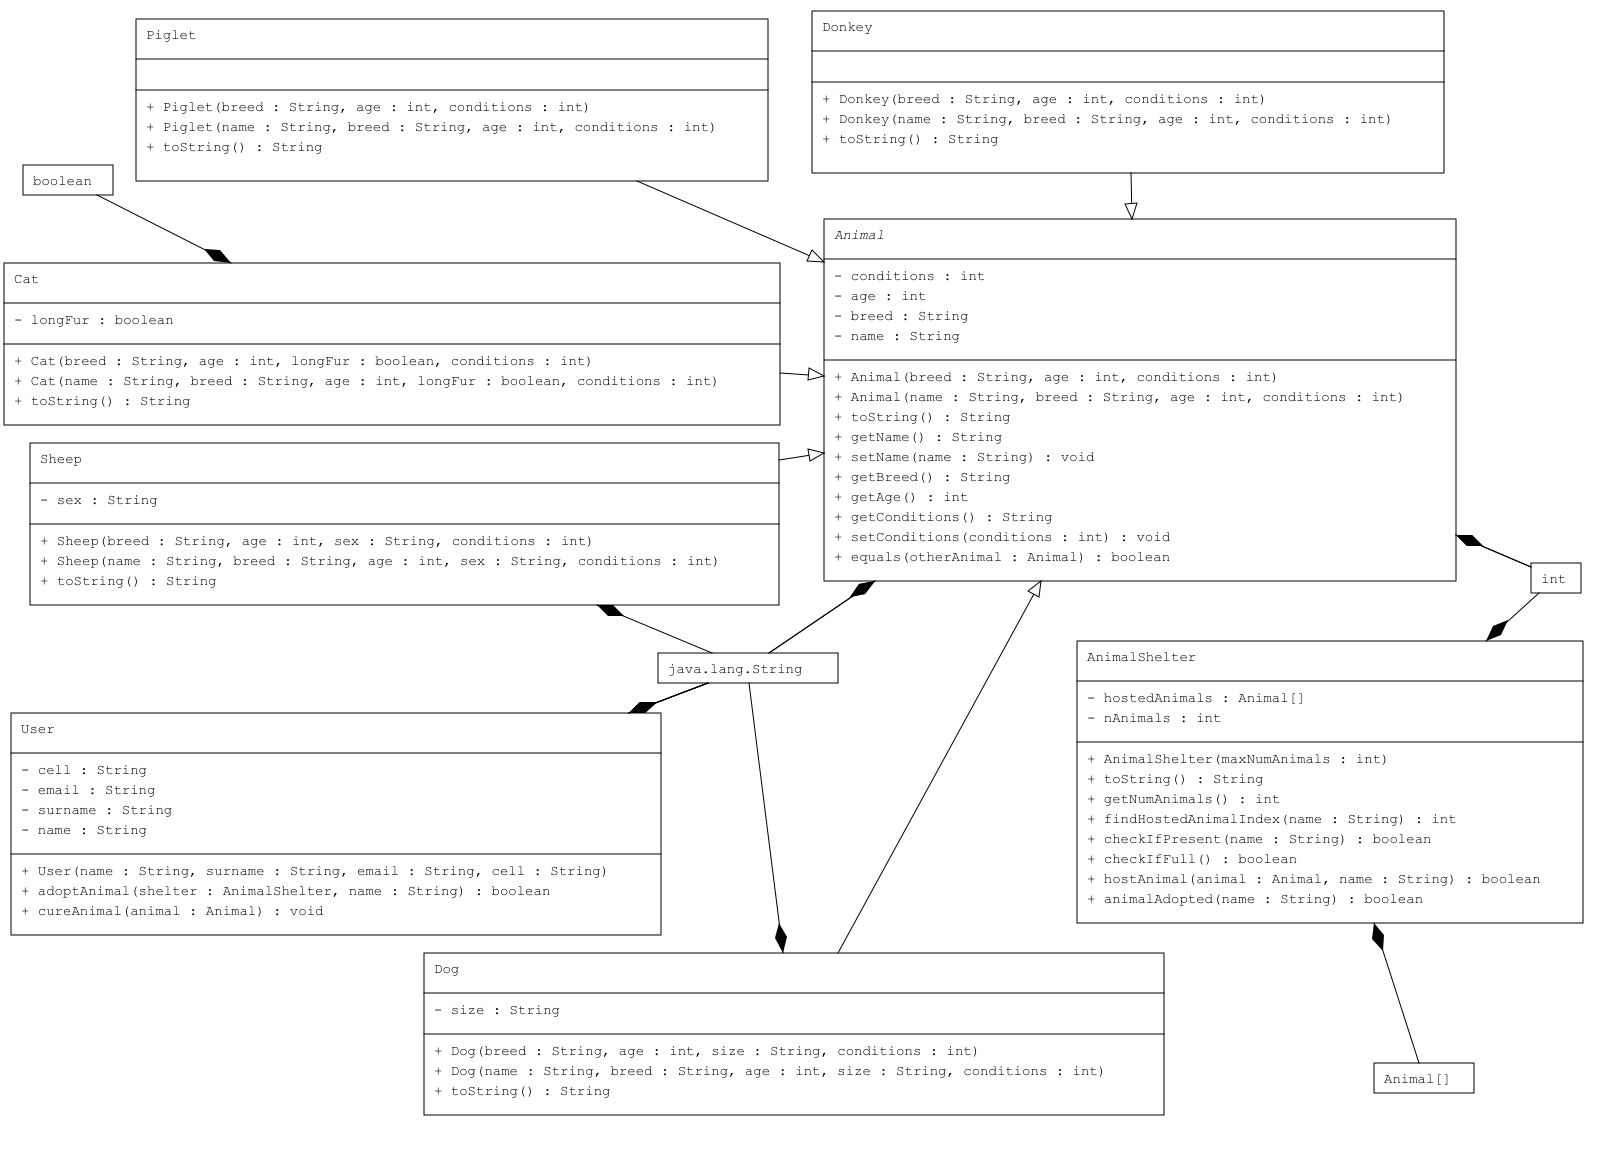
\includegraphics[width=1.2\linewidth]{immagini/uml_base.png}}
  \caption{\small Interconnessione delle classi implementate mostrata come diagrammi UML.}
  \label{fig:UML}
\end{figure}


\newpage
\printbibliography


\newpage
\appendix
\section{Codice Sorgente}
\label{appendice:A}

\begin{lstlisting}[caption={Animal.java}]
// Definendo Animal come astratta posso usare il Binding Dinamico 
// per astrarre lo shelter come un array di tipo
// apparente Animal, ma di tipo esatto quello specifico della specie 
// che estende la classe astratta Animal.
abstract class Animal {
private String name, breed;
private int age, conditions; // condizioni di salute dell'animale adottato

public Animal(String breed, int age, int conditions) {
  this.breed = breed;
  this.age = age;
  this.conditions = conditions;
}

// OVERLOADING: ridefinisco il costruttore della classe Animal 
// per accettare anche l'inizializzazione del campo "name"
public Animal(String name, String breed, int age, int conditions) {
  this.name = name;
  this.breed = breed;
  this.age = age;
  this.conditions = conditions;
}

// Converto l'astrazione dell'animale in una stringa. OVERWRITING: ridefinisco il metodo toString() della classe Object
public String toString() {
  String s = "\n nome: " + name + ", razza: " + breed + ", eta': " + age + ", condizioni generali: " + conditions + "%";
  return s;
}

public String getName() {
  return name;
}

public void setName(String name) {
  this.name = name;
}

public String getBreed() {
  return breed;
}

public int getAge() {
  return age;
}

public String getConditions() {
  return name;
}

public void setConditions(int conditions) {
  this.conditions = conditions;
}

// Il metodo equals() fa parte dei metodi "standard" delle librerie Java, lo ridefinisco perchè mi serve definire
// un concetto di uguaglianza tra gli animali.
public boolean equals(Animal otherAnimal) {
  // Per definire l'uguaglianza uso i campi comuni a tutti gli animali. Tali campi rendono univoco il
  // riconoscimento di un animale ospitato nello shelter
  return
          (this.name.equalsIgnoreCase(otherAnimal.name))
                  &&
                  (this.breed.equalsIgnoreCase(otherAnimal.breed))
                  &&
                  (this.age == otherAnimal.age);
}
}


class Dog extends Animal {

// Subclasses add more feature alla classe che specializzano
private String size;

public Dog(String breed, int age, String size, int conditions) {
  super(breed, age, conditions);
  this.size = size;
}

public Dog(String name, String breed, int age, String size, int conditions) {
  super(name, breed, age, conditions);
  this.size = size; // NB: this esplicito
}

// OVERWRTING del metodo toString()
public String toString() {
  String s = super.toString() + ", taglia: " + size + ", animale: cane"; // NB: this implicito

  return s;
}
}


class Cat extends Animal {
private boolean longFur;

public Cat(String breed, int age, boolean longFur, int conditions) {
  super(breed, age, conditions);
  this.longFur = longFur;
}

public Cat(String name, String breed, int age, boolean longFur, int conditions) {
  super(name, breed, age, conditions);
  this.longFur = longFur;
}

public String toString() {
  String s = super.toString() + ", pelo lungo: " + longFur + ", animale: gatto";;

  return s;
}
}


class Sheep extends Animal {
private String sex;

public Sheep(String breed, int age, String sex, int conditions) {
  super(breed, age, conditions);
  this.sex = sex;
}

public Sheep(String name, String breed, int age, String sex, int conditions) {
  super(name, breed, age, conditions);
  this.sex = sex;
}

public String toString() {
  String s = super.toString() + ", sesso: " + sex + ", animale: pecora";

  return s;
}
}


class Donkey extends Animal {

public Donkey(String breed, int age, int conditions) {
  super(breed, age, conditions);
}

public Donkey(String name, String breed, int age, int conditions) {
  super(name, breed, age, conditions);
}

public String toString() {
  String s = super.toString() + ", animale: asino";

  return s;
}
}


class Piglet extends Animal {
public Piglet(String breed, int age, int conditions) {
  super(breed, age, conditions);
}

public Piglet(String name, String breed, int age, int conditions) {
  super(name, breed, age, conditions);
}

public String toString() {
  String s = super.toString() + ", animale: maialino";

  return s;
}
}⏎  
\end{lstlisting}

\begin{lstlisting}[caption = {User.java}]
public class User {
private String name;
private String surname;
private String email;
private String cell;

public User(String name, String surname, String email, String cell){
  this.name = name;
  this.surname = surname;
  this.email = email;
  this.cell = cell;
}

public boolean adoptAnimal(AnimalShelter shelter, String name){
  return shelter.animalAdopted(name);
}

public void cureAnimal(Animal animal){
  animal.setConditions(100);
}
}⏎ 
\end{lstlisting}

\begin{lstlisting}[caption={AnimalShelter.java}]
public class AnimalShelter {

private int nAnimals = 0; // inizialmente lo shelter non contiene animali
private Animal[] hostedAnimals;

// Definisco lo shelter come un array di oggetti, quindi avente una capienza limitata a maxNumAnimals
public AnimalShelter(int maxNumAnimals) {
  hostedAnimals = new Animal[maxNumAnimals];
}

// Converto l'astrazione dell'AnimalShelter in una stringa. Notare la chiamata al metodo toString della classe Animal.
public String toString() {
  String s = "Numero di animali ospitati = " + nAnimals;

  int i = 0;
  while (i < nAnimals) {
     s = s + hostedAnimals[i].toString();
     ++i;
  }

  return s;
}

public int getNumAnimals() {
  return nAnimals;
}

public int findHostedAnimalIndex(String name) {
  int i = 0;
  while (i < nAnimals) {
     if (hostedAnimals[i].getName().equalsIgnoreCase(name)) return i;
     ++i;
  }

  return nAnimals;
}

public boolean checkIfPresent(String name) {
  return (findHostedAnimalIndex(name) < nAnimals);
}

public boolean checkIfFull() {
  return (nAnimals == hostedAnimals.length);
}

public boolean hostAnimal(Animal animal, String name) {

  if (checkIfFull()){
     return false; // Se lo shelter è pieno il motodo fallisce
  }

  animal.setName(name);
  hostedAnimals[nAnimals] = animal;
  ++nAnimals; // aggiorno il numero degli animali presenti

  return true;
}

public boolean animalAdopted(String name) {
  int i = findHostedAnimalIndex(name);
  if (i == nAnimals) {
     return false; // se l'animale non esiste il motodo fallisce
  }

  --nAnimals;
  hostedAnimals[i] = hostedAnimals[nAnimals];

  return true;
}
}⏎  
\end{lstlisting}

\begin{lstlisting}[caption={DemoAnimalShelter.java}]
public class DemoAnimalShelter {
public static void main(String arg[]) {

  // Inizializzo un utente
  User Mila = new User("Mila", "Racca", "Mila.Racca@me.it", "+39 377 24583");
  User Piero = new User("Piero", "Gillono", "Piero.Gillono@me.it", "+39 347 58232");

  // Inizializzo lo shelter definendo il nume di posti che dispone per ospitare gli animali
  AnimalShelter shelter = new AnimalShelter(100);

  Animal dog1 = new Dog("Labrador", 6, "mid", 90);
  Animal dog2 = new Dog("Bassotto", 6, "small", 80);
  Animal cat1 = new Cat("European", 5, false,85);
  Animal cat2 = new Cat("Siamese", 2, true,33);
  Animal sheep1 = new Sheep("Irlandese", 4, "female",95);
  Animal sheep2 = new Sheep("Yorkshire", 4, "female",60);
  Animal sheep3 = new Sheep("British Columbia", 4, "male",70);
  Animal donkey1 = new Donkey("Sarda", 10,90);

  // Ospitando un animale, gli assegno un nome :)
  shelter.hostAnimal(dog1, "Buddy");
  shelter.hostAnimal(dog2, "Otto von Bismarck");
  shelter.hostAnimal(cat1, "Tom");
  shelter.hostAnimal(cat2, "Dorotea");
  shelter.hostAnimal(sheep1, "Margarita");
  shelter.hostAnimal(sheep2, "Jimmy");
  shelter.hostAnimal(sheep3, "Ed");
  shelter.hostAnimal(donkey1, "Arturo");

  System.out.println("\nSituazione dello shelter a un mese dall'apertura:\n" + shelter);

  System.out.println("\nOtto von Bismarck è ospitato nello shelter: " + shelter.checkIfPresent("Otto von Bismarck"));

  Mila.adoptAnimal(shelter, "Otto von Bismarck");

  System.out.println("Otto von Bismarck viene adottato. \nOtto von Bismarck è ospitato nello shelter: " + shelter.checkIfPresent("Otto von Bismarck"));

  System.out.println("\nIl veterinario riesce a curare i due gatti presenti in struttura.");
  Piero.cureAnimal(cat1);
  Piero.cureAnimal(cat2);

  System.out.println("\nSituazione dello shelter:\n" + shelter);
}
}⏎   
\end{lstlisting}
	
\begin{figure}[!t]
    \makebox[\textwidth][c]{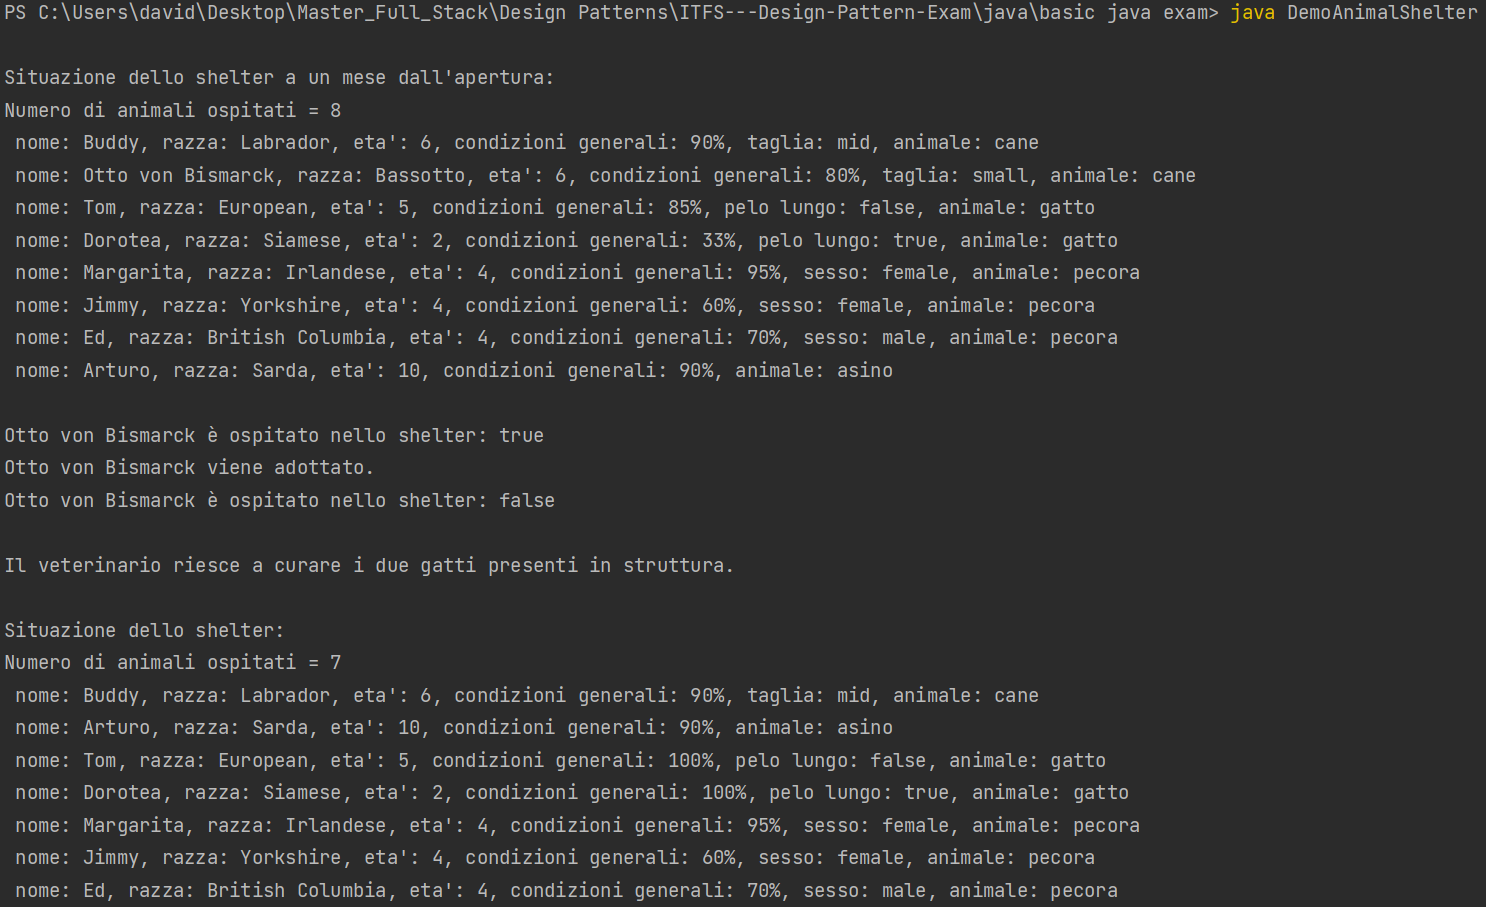
\includegraphics[width=1.1\linewidth]{immagini/output_base.png}}
  \caption{\small L'output del client.}
  \label{fig:output}
\end{figure}
	
\end{document}